\documentclass[9pt]{article}
\usepackage{multicol}
\usepackage{graphicx}
\linespread{1.35}
\usepackage{amsmath}
\usepackage{color}
\usepackage{xcolor}
\usepackage{tikz}
\usetikzlibrary{arrows,automata}


\begin{document}

\begin{flushright}
 \texttt{Regular Expression} \hspace*{0.10cm}\textbf{$|$} \textbf{229}\hspace*{0.5cm}
\end{flushright}

\vspace*{0.5cm}
(Putting the value of R in the LHS, we get)\\

\vspace*{0.2cm}
\hspace*{4cm} $QP* - Q - QP* P$ \\
\hspace*{4cm} $= QP* - Q(^ + P* P)$ \\
\hspace*{4cm} $= QP* - QP* [As (\Lambda + R*R) = R*]$ \\
\hspace*{4cm} $= 0.$ \\

\vspace*{0.2cm}
So, from here it is proved that $R = QP*$ is a solution of the equation $R = Q + RP.$ \\
Now, we have to prove that $R = QP*$ is the one and only solution of the equation $R = Q + RP$. \\
As $R = Q + RP$, put the value of R again and again in the RHS of the equation.\\
\vspace*{0.2cm}

\hspace*{3.1cm} $R = Q + RP$ \\
\hspace*{3.5cm} $= Q + (Q + RP)P$ \\
\hspace*{3.5cm} $= Q + QP + RPP$ \\
\hspace*{3.5cm} $= Q(\Lambda + P) + RPP$ \\
\hspace*{3.5cm} $= Q(\Lambda + P) + (Q + RP)PP$ \\
\hspace*{3.5cm} $= Q(\Lambda + P) + QPP + RPPP$ \\
\hspace*{3.5cm} $= Q(\Lambda + P + PP) + RPPP.$ \\
\vspace*{0.1cm}

After several steps, we shall get\\

\vspace*{0.1cm}
\hspace*{3cm} $R = Q(\Lambda + P + P^2 + P^3 + .... P^n) + RP^n + 1.$ \\

\vspace*{0.1cm}
\hspace*{0.5cm} Now let a string w belong to R. If w is a $\Lambda$ string, then in which part will the $\Lambda$ belong?\\


\hspace*{0.5cm} This string will belong to either the $Q(\Lambda + P + P^2 + P^3 + .... P^n)$ part or the $RP^n + 1$ part. But, according
to point number (ii), P does not contain $\Lambda$, and so the string w does not belong to $RP^n + 1$. So, it will
obviously belong to $Q(\Lambda + P + P^2 + P^3 + .... P^n)$ which is nothing but $QP*. [(\Lambda + P + P^2 + P^3 + .... P^n)$ is
any combination of P including $\Lambda$.]\\

\hspace*{0.5cm} As this string belongs only in one part, R and QP* represent the same set. That means $R = QP*$ is the
unique solution of the equation $R = Q + RP.$\\

\vspace*{0.5cm}
\large{
\textbf{5.4.1 Process of Constructing Regular Expression\\
\hspace*{0.7cm} from Finite Automata}\\
}

\vspace*{0.2cm}

There are some assumptions:\\

\vspace*{0.1cm}
\begin{itemize}
  \item In the transitional graph, there must be no $\Lambda$-move.\\
  \item In the FA, there is only one initial state.\\

  \vspace*{0.1cm}
\hspace*{0.5cm} Now, we have to construct equations for all the states. There are n number of equations if there are
n-states.\\
\hspace*{0.5cm} For any FA, these equations are constructed in the following way.\\

\vspace*{0.1cm}
\hspace*{1cm} $<$ State name $> = \Sigma [<$ State name from which inputs are coming $>. < input >]$ \\

\vspace*{0.1cm}
For the beginning state, there is an arrow at the beginning coming from no state. So, a $\Lambda$ is added with
the equation of the beginning state.\\
\end{itemize}

\newpage
\begin{flushleft}
    \textbf{230}\hspace*{0.1cm} \textbf{$|$} \hspace*{0.1cm} \texttt{Introduction to Automata Theory, Formal Languages and Computation}
  \end{flushleft}

\vspace*{0.3cm}

\hspace*{0.5cm} Then, these equations have to be solved by the identities of RE.The expression obtained for the final
state and consists of only the input symbol $(\Sigma)$ is the Regular Expression for the Finite Automata.\\
\hspace*{0.5cm} The following examples describe the process of the construction of an RE from FA.\\

\fcolorbox{red}{blue}{\textbf{\textcolor[rgb]{1.00,1.00,1.00}{Example 5.6}}}\hspace*{0.1cm} \texttt{\small{Construct an RE from the given FA in Fig. 5.1 by the algebraic method using Arden’s theorem}} \\

\begin{center}
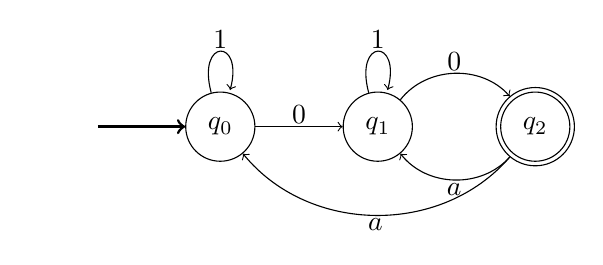
\begin{tikzpicture}[node distance = 2cm,auto,inner sep=1pt]
\node[state,draw=white,inner sep=0pt] (A) {$$};
\node[state,draw=black] (B) [ right of = A]  {$q_0$};
\node[state,draw=black] (C) [right of = B]  {$q_1$};
\node[state,draw=black] (D) [right of = C]  {$q_2$};
\node[state,draw=black,inner sep=10pt] (E) [right of = C]  {$$};

\path (A) edge [->,line width=1pt,node distance = 0.1cm] node {$$} (B);
\path (B) edge [->] node {$0$} (C);
\path (B) edge [->,loop above] node {$1$} (B);
\path (C) edge [->,loop above] node {$1$} (C);
\path (C) edge [->,bend left=50] node {$0$} (E);
\path (E) edge [->,bend left=50] node {$a$} (C);
\path (E) edge [->,bend left=50] node {$a$} (B);

\end{tikzpicture}
\end{center}
\begin{center}
\textbf{Fig. 5.1}
\end{center}

\textbf{Solution:}\\
\hspace*{0.5cm} For the previously given FA, the equations are\\

\hspace*{3.5cm} $q_0 = q_0.1 + q_2.1 + \Lambda$   \hspace*{3.5cm} (1) \\
\hspace*{4cm} $q_1 = q_0.0 + q_1.1 + q_2.0$     \hspace*{2.7cm} (2) \\
\hspace*{4cm} $q_2 = q_1.0$                     \hspace*{5.6cm} (3) \\

\hspace*{0.5cm} Put the value of $q_2$ in equation no. (2).\\
\hspace*{4cm} $q_1 = q_0.0 + q_1.1 + q_1.0.0$ \\
\hspace*{4.4cm} $= q_0.0 + q_1(1 + 0.0)$  \hspace*{2.7cm} (4)\\

\vspace*{0.1cm}
\hspace*{0.5cm} This equation is in the form $R = Q + RP$, where $R = q_1, Q = q_0.0$, and $P = (1 + 0.0)$.\\
\hspace*{0.5cm} So, the solution of the equation is $R = QP^*, i.e., q_1 = q_0.0. (1 + 0.0)^*$.\\
\hspace*{0.5cm} Putting the value $q_2 = q_1.0$ in equation no. (1), we get\\

\vspace*{0.1cm}
\hspace*{4.4cm} $q_0 = q_0.1 + q_1.0.1 + \Lambda.$ \\

\vspace*{0.1cm}

\hspace*{0.5cm} Again putting the value of $q_1$ in the previous equation, we get\\

\vspace*{0.1cm}
\hspace*{3cm} $q_0 = q_0.1 + q_0.0. (1 + 0.0)^*.0.1 + \Lambda$ \\

\hspace*{3cm} $q_0 = q_0(1 + 0.(1 + 0.0)^*.0.1) + \Lambda.$ \\

\vspace*{0.1cm}
\hspace*{0.5cm} This equation is in the form $R = Q + RP$, where $R = q_0, Q = \Lambda$, and $P = (1 + 0.(1 + 0.0)^*.0.1)$. So, the
solution of the equation is\\

\hspace*{3cm} $q_0 = \Lambda.(1 + 0.(1 + 0.0)^*.0.1)^*$ \\
\hspace*{3.4cm} $= (1 + 0.(1 + 0.0)^*.0.1)^*.$ \\

\vspace*{0.1cm}
Putting the value of $q_0$ in the solution of $q_1$, we get\\
\vspace*{0.1cm}

\hspace*{2.5cm} $q_1 = (1 + 0.(1 + 0.0)^*.0.1)^*.0. (1 + 0.0)^*.$ \\

\newpage
\begin{flushleft}
    \textbf{230}\hspace*{0.1cm} \textbf{$|$} \hspace*{0.1cm} \texttt{Introduction to Automata Theory, Formal Languages and Computation}
  \end{flushleft}

  \vspace*{0.5cm}

 \hspace*{0.5cm} Replacing the value of $q_1$ in equation (3), we get\\

\hspace*{2.5cm} $q_2 = (1 + 0.(1 + 0.0)^*.0.1)^*.0. (1 + 0.0)^*.0.$ \\


 \hspace*{0.5cm} As q2 is the final state of the FA, all the strings will halt on this state. Therefore, the RE is $(1 + 0.
(1 + 0.0)^*.0.1)^*.0. (1 + 0.0)^*.0$, thus accepting the FA.\\

\fcolorbox{red}{blue}{\textbf{\textcolor[rgb]{1.00,1.00,1.00}{Example 5.7}}}\hspace*{0.1cm} \texttt{\small{Construct an RE from the given FA in Fig. 5.2 by the algebraic method using Arden’s theorem.}} \\

\begin{center}
\section{picture}
\includegraphics[width=6cm,height=3cm]{231.png}
\end{center}


\textbf{Solution:} For the previously given FA, the equations are\\

\hspace*{4cm} $q_0 = \Lambda$ \hspace*{5.2cm} (1)\\
\hspace*{4cm} $q_1 = q_00 + q_10$ \hspace*{4.2cm}  (2)\\
\hspace*{4cm} $q_2 = q_11 + q_21$ \hspace*{4.1cm}  (3)\\
\hspace*{4cm} $q_3 = q_20 + q_01 + q_3 (0 + 1)$  \hspace*{2cm}   (4)\\

 \vspace*{0.1cm}
Putting the value of $q_0$ in equation $q_1$, it becomes $q_1 = 0 + q_10$. The equation is in the form $R = Q +
RP$, where $R = q_1, Q = 0$, and $P = 0$. By the Arden’s theorem, the solution of the equation is $R = QP^*, i.e.$,\\

 \vspace*{0.1cm}
\hspace*{5cm} $q_1 = 00^*$.\\
 \vspace*{0.1cm}

 \hspace*{0.5cm} Putting the value of $q_1$ in the equation (3), we get $q2 = 00^*1 + q21$.\\
 \hspace*{0.5cm} The equation is in the form $R = Q + RP$, where $R = q_2, Q = 00^*1$, and $P = 1$. By the Arden’s theorem,
the solution of the equation is $R = QP^*$, i.e.,\\

 \vspace*{0.1cm}

\hspace*{4.5cm} $q_2 = 00^*11^*$.\\
 \vspace*{0.1cm}

 \hspace*{0.5cm} Putting the value of $q_2$ and $q_0$ in equation (4), we get\\

 \vspace*{0.1cm}
\hspace*{3cm} $q_3 = (00^*11^*0 + 1) + q_3 (0 + 1)$.\\

 \vspace*{0.1cm}
The equation is in the form $R = Q + RP$, where $R = q_3, Q = (00^*11^*0 + 1)$, and $P = (0 + 1)$. By the
Arden’s theorem, the solution of the equation is $R = QP*$, i.e.,\\

 \vspace*{0.1cm}
\hspace*{3.2cm} $q_3 = (00^*11^*0 + 1) (0 + 1)^*$.\\
 \vspace*{0.1cm}

 \hspace*{0.5cm} As $q_3$ is the final state, the RE generated from the given FA is $(00^*11^*0 + 1) (0 + 1)^*$.\\

\newpage
\begin{flushleft}
    \textbf{232}\hspace*{0.1cm} \textbf{$|$} \hspace*{0.1cm} \texttt{Introduction to Automata Theory, Formal Languages and Computation}
  \end{flushleft}

\vspace*{0.3cm}
\fcolorbox{red}{blue}{\textbf{\textcolor[rgb]{1.00,1.00,1.00}{Example 5.8}}}\hspace*{0.1cm} \texttt{\small{Construct an RE from the given FA in Fig. 5.3 by the algebraic method using Arden’s theorem}}\\

\begin{center}
\section{picture}
\includegraphics[width=6cm,height=3cm]{232-1.png}
\end{center}


\textbf{Solution:} For the given FA, the equations are\\

\vspace*{0.1cm}
\hspace*{4cm} $q_1 = q_21 + q_30 + \Lambda$  \hspace*{3.4cm}  (1) \\
\hspace*{4cm} $q_2 = q_10$  \hspace*{4.7cm}  (2) \\
\hspace*{4cm} $q_3 = q_11$  \hspace*{4.7cm}  (3) \\


\hspace*{0.3cm} Substituting the value of $q_2$ and $q_3$ in $q_1$, we get\\

\vspace*{0.1cm}
\hspace*{4cm} $q_1 = q_1^01 + q_1^10 + \Lambda$ \\
\hspace*{4cm} $q_1 = q_1(01 + 10) + \Lambda.$ \\

\vspace*{0.1cm}
If $q_1$ is treated as R, $\Lambda$ as Q, and $(01 + 10)$ as P, then the equation becomes $R = Q + RP$.
The solution for the equation is $R = QP^*$.\\

\vspace*{0.1cm}
So, \hspace*{1.5cm}  $q_1 = \Lambda(01 + 10)^*, i.e., q_1 = (01 + 10)^* (As \Lambda.R = R)$.\\

\vspace*{0.1cm}
\hspace*{0.5cm} As $q_1$ is the only final state, the string accepted by the FA is $(01 + 10)^*$.\\

\hspace*{0.5cm}(Note: In the automata the transition from $q_2$ and $q_3$ for input 1 is missing. A dead state may be added
to complete this FA, but the equation for dead state will be in no need in solving the automata. From
here, it is also proved that the dead state is only necessary to prove that a string is not accepted by an FA
by totally traversing the string.)\\

\vspace*{0.2cm}
\fcolorbox{red}{blue}{\textbf{\textcolor[rgb]{1.00,1.00,1.00}{Example 5.8}}}\hspace*{0.1cm} \texttt{\small{Construct an RE from the given FA in Fig. 5.4 by the algebraic method using Arden’s theorem.}} \\

\vspace*{0.1cm}
\begin{center}
\section{picture}
\includegraphics[width=6cm,height=3cm]{232-2.png}
\end{center}


\end{document}

